\documentclass{sigchi}

% Use this section to set the ACM copyright statement (e.g. for
% preprints).  Consult the conference website for the camera-ready
% copyright statement.

% Copyright
\CopyrightYear{2016}
%\setcopyright{acmcopyright}
\setcopyright{acmlicensed}
%\setcopyright{rightsretained}
%\setcopyright{usgov}
%\setcopyright{usgovmixed}
%\setcopyright{cagov}
%\setcopyright{cagovmixed}
% DOI
\doi{http://dx.doi.org/10.475/123_4}
% ISBN
\isbn{123-4567-24-567/08/06}
%Conference
\conferenceinfo{CHI'16,}{May 07--12, 2016, San Jose, CA, USA}
%Price
\acmPrice{\$15.00}


% Load basic packages
\usepackage{balance}       % to better equalize the last page
\usepackage{graphics}      % for EPS, load graphicx instead 
\usepackage[T1]{fontenc}   % for umlauts and other diaeresis
\usepackage{txfonts}
\usepackage{mathptmx}
\usepackage[pdflang={en-US},pdftex]{hyperref}
\usepackage{color}
\usepackage{booktabs}
\usepackage{textcomp}

% Some optional stuff you might like/need.
\usepackage{microtype}        % Improved Tracking and Kerning
% \usepackage[all]{hypcap}    % Fixes bug in hyperref caption linking
\usepackage{ccicons}          % Cite your images correctly!
% \usepackage[utf8]{inputenc} % for a UTF8 editor only

% If you want to use todo notes, marginpars etc. during creation of
% your draft document, you have to enable the "chi_draft" option for
% the document class. To do this, change the very first line to:
% "\documentclass[chi_draft]{sigchi}". You can then place todo notes
% by using the "\todo{...}"  command. Make sure to disable the draft
% option again before submitting your final document.
\usepackage{todonotes}

% Paper metadata (use plain text, for PDF inclusion and later
% re-using, if desired).  Use \emtpyauthor when submitting for review
% so you remain anonymous.
\def\plaintitle{ForceScroll: Enhance Reading Speed Using Force Touch Technique}
\def\plainauthor{First Author, Second Author, Third Author,
  Fourth Author, Fifth Author, Sixth Author}
\def\emptyauthor{}
\def\plainkeywords{Human Computer Interaction; Trackpad; Force Touch; Experiment.}
\def\plaingeneralterms{Documentation, Standardization}

% llt: Define a global style for URLs, rather that the default one
\makeatletter
\def\url@leostyle{%
  \@ifundefined{selectfont}{
    \def\UrlFont{\sf}
  }{
    \def\UrlFont{\small\bf\ttfamily}
  }}
\makeatother
\urlstyle{leo}

% To make various LaTeX processors do the right thing with page size.
\def\pprw{8.5in}
\def\pprh{11in}
\special{papersize=\pprw,\pprh}
\setlength{\paperwidth}{\pprw}
\setlength{\paperheight}{\pprh}
\setlength{\pdfpagewidth}{\pprw}
\setlength{\pdfpageheight}{\pprh}

% Make sure hyperref comes last of your loaded packages, to give it a
% fighting chance of not being over-written, since its job is to
% redefine many LaTeX commands.
\definecolor{linkColor}{RGB}{6,125,233}
\hypersetup{%
  pdftitle={\plaintitle},
% Use \plainauthor for final version.
%  pdfauthor={\plainauthor},
  pdfauthor={\emptyauthor},
  pdfkeywords={\plainkeywords},
  pdfdisplaydoctitle=true, % For Accessibility
  bookmarksnumbered,
  pdfstartview={FitH},
  colorlinks,
  citecolor=black,
  filecolor=black,
  linkcolor=black,
  urlcolor=linkColor,
  breaklinks=true,
  hypertexnames=false
}

% create a shortcut to typeset table headings
% \newcommand\tabhead[1]{\small\textbf{#1}}

% End of preamble. Here it comes the document.
\begin{document}

\title{\plaintitle}

\numberofauthors{2}
\author{%
  \alignauthor{Ruoteng Ma\\
    \affaddr{University of Waterloo}\\
    \affaddr{Waterloo, Canada}\\
    \email{ruoteng.ma@uwaterloo.ca}}\\
  \alignauthor{Sung-Shine Lee\\
    \affaddr{University of Waterloo}\\
    \affaddr{Waterloo, Canada}\\
    \email{s469lee@uwaterloo.ca}}
}




\maketitle

\begin{abstract}
  With the increasing availability of digital literatures, reading using digital devices have became common practice. While mobile devices removed the need of carrying physical books, navigating through a digital document can also be a challenging task. Without the help of mouse and physical keyboard, digital devices usually rely on trackpad interactions to enable navigation. In recent years, a number of devices have started to take the amount of forces applied during the trackpad interaction into consideration. In this paper, we present ForceScroll, a novel interaction technique that utilizes the new interaction dimensions added by force touch to improve the interaction experience provided by the traditional trackpad control scheme. The system will be implemented using JavaScript. We present a series of experiments comparing the ForceScroll against traditional trackpad control technique, in which we examine the error rate and efficiency of the new system. The main contribution of paper is to propose a new interaction technique that is more efficient than the existing technique.  
\end{abstract}

\category{H.5.2.}{Information Interfaces and Presentation
  (e.g. HCI)}{User Interfaces
  - Input devices and strategies} \category{}{}{}

\keywords{\plainkeywords}

\section{Introduction}

Book readers use their fingers to turn the pages of the book they are reading, they can easily control the amount of pages they are turning and quickly reach desired location. A larger amount of existing literatures are presented as digital documents, readable on devices such as Personal Computers and Laptops. For reading digital documents on these devices, the task of efficiently moving between pages and find desired contents can be difficult to achieve. Personal computers and laptops allow users to control their devices using physical keyboard and mouse, this gives user a reliable and easy way to navigate the document. However, problem arises for laptop users without access to mouse, who perform their interaction using trackpad. Without the support of physical mouse, viewing documents on these devices can be inefficient. 

%Different types of digital documents also provide different ways of traversal. Documents with well defined pages could be traversed by going directly to a specified page; documents that have a table-of-contents which is linked to well-defined sections allow users to go directly to desired chapter or section of the document, regardless of the length of the document; documents without any of the above functions will need to be traversed by moving through the entire document sequentially. 


ForceScroll presents an alternative control scheme for devices that support force-sensitive trackpad. We want to design a new viewing control scheme for these devices by applying force touch. We believe that with the help of force touch, the efficiency of trackpad control can be improved. 


Digital documents can also have different designs and functionalities. For ForceScroll, we assume all documents viewed on the device have well-defined and linked pages and sections, which allows users to jump to certain location within the document. For the purpose of evaluation the new technique, we are only interested in the improvement ForceScroll system has on the Scrolling gesture performed on trackpads. To test the ForceScroll system in a controlled environment, we do not consider other page turning methods, such as entering a page number or using the table-of-content. We implemented the prototype system on a Macbook laptop with force-sensitive trackpad.    
  

Force touch has been explored by a number of works, Presstures \cite{rendl2014presstures} allows users to apply force to select interaction mode in order to avoid uncomfortable interactions such as pressing hard for a long distance. Heo and Lee \cite{heo2011force} designed a web browser and an e-book reader that both use force input as the main control technique and give users visual feedback on the applied force. ForceEdge \cite{antoine2017forceedge} expends the autoscroll function on touch devices with force-sensing ability, resulting in a more accurate target-seeking experience. Surale et al. \cite{surale2017experimental} explored mode-switching task with six gestures both with and without force, Taher et al. \cite{taher2014empirical} studied the characterization of input force on mobile devices and provided a baseline for further studies. Finally, Mandalapu and Subramanian \cite{mandalapu2011exploring} explored the idea of using force as an alternative to multi touch interactions. ForceScroll benefits from previous studies, but in the context of document viewing, there is a lack of comparison between force-enabled techniques and traditional techniques, and our interaction system is different from those proposed before.          


ForceScroll allows readers to control the page scrolling process in two ways. A simple swipe movement perform the traditional scrolling operation, where the location of on-screen content moves according to the distance and speed of the movement. A swipe with force applied moves the on screen content to the next chapter or section. We built the ForceScroll application using JavaScript, the application achieves the above functionality and allows us to test our hypothesis in a controlled environment. We evaluate the system by the time required for a user to reach a target location and the rate of error, note that more evaluation criteria may be added as the project progresses. See Figure 1 for an illustration.  


\begin{figure}[!h]
	\centering
	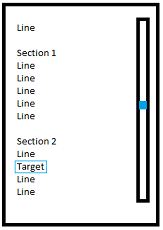
\includegraphics[width=0.6\columnwidth]{figures/Capture}
	\caption{The participants were required to move the screen until the highlighted target was on screen and click it. The general location of the target in the document might also be displaced on a sidebar}~\label{fig:figure1}
\end{figure}

ForceScroll also provides the users with a visual feedback for the level of force applied. Although the format of feedback have not yet been decided as of now.

The main contribution of ForceScroll is that we propose a novel interaction technique that utilizes the power of force touch to facilitate the page scrolling task for trackpad devices, we also performed a comparison study between the new technique and the traditional technique where force sensing is disabled.

\section{Related Work}

\subsection{Scrolling}
As one of the most commonly used features on digital devices, scrolling as an operation has been thoroughly studied. Andersen \cite{andersen2005simple} developed a linear model for the scrolling movement time with an optical mouse and distance to target, and concluded that the scrolling movement time does not follow Fitts' law. Quinn et al. \cite{quinn2012exposing} acknowledged the difficulty in studying scrolling operation since the existing transfer functions, which can be used to alter scrolling performance, are unknown to researchers. They created a framework of transfer function factors and proposed a method to study proprietary transfer functions for different input devices. Cockburn et al. \cite{cockburn2012improving} presented three gain functions, called document-length-dependent gain, which utilize document length as an input of the function, to improve scrolling performance. Aceituno et al. \cite{aceituno2017design} studied the performance of different edge-scrolling techniques and presented a framework of factors that affect performance and design.  

A variety of alternative scrolling methods have been proposed and studied. For example, Smith and Schraefel \cite{smith2004radial} presented the radial scroll interface, which allows users to scroll up and down by performing clock and counter-clockwise gestures on a touch interface. Other than simple alternative interaction gestures, some works aimed to extend the interaction space. Takashima et al. \cite{takashima2015exploring} proposed an improved scrolling control by extending the motor space of the action. Their interface can be applied on touch devices, using either off-window touch space or mid-air motions detectable by 3D motion sensors. Push-Edge \cite{malacria2015push} detected cursor at the edge of the viewport, it captured device signals from action space outside the viewport and used them as input to a scrolling transfer function, thus altered the traditional edge-scrolling feature and kept the cursor stationary on the screen while scrolling. Other studies attempted to expend the dimension of the interaction. Miyaki and Rekimoto \cite{miyaki2009graspzoom} proposed a pressure sensing interaction technique, GraspZoom, for the scrolling task on mobile devices with an attached Force Sensitive Resistor on the back of the device. The utilization of pressure increased the dimension of interaction and allowed gestures to be augmented by pressure.  

Research has also been done on scrolling task with a focus on the trackpad. Bial et al. \cite{bial2010study} proposed a two-handed input scheme, where the trackpad was used as a dedicated scrolling device. The system also implemented different scrolling actions such as relative scrolling and flicking. Arthur et al. \cite{arthur2008evaluating} also presented a circular touch gesture called ChiralMotion that can be performed on the trackpad. The system reduces 2D motions to 1D scrolling actions.


\subsection{Force Touch}
In this section, we discuss previous works on force sensitive touch input. Taher et al. \cite{taher2014empirical} derived a ground-truth characterization of force touch gestures by performing a controlled user study; this gives a good starting point for designing input scheme using the force-sensitive technique. 


The applications of force on traditional interaction methods have been proposed and studied by many authors. Goguey et al. \cite{goguey2018improving} designed a force-sensitive text selection system that allowed different actions for each level of pressure applied. By applying different levels of force before releasing their finger, the system lets users select different portions of text centered around the touched position. Zoofing \cite{quinn2009zoofing} presented a pressure-based zooming technique as a part of their list selection interface where the level of zooming was controlled by the level of pressure applied at the zoom point. Also focused on zooming, Mandalapu and Subramanian \cite{mandalapu2011exploring} explored the possibility of using pressure as an alternative to multi-touch control. ForceEdge \cite{antoine2017forceedge} explored the use of force for trackpad autoscrolling, allowing users to control the scrolling rate by varying applied force. Heo and Lee \cite{heo2011force} presented a system that augmented traditional touchscreen gestures with two levels of force, where the same gesture invoked different actions when the amount of force applied was different. They also designed two sample applications for their system. Their work is closely related to ForceScroll. 

Many research studied the effect of visualized feedback since the force touch systems could support different functionalities for different levels of force applied. Sheik-Nainar et al. \cite{sheik2013two} developed an interaction model for their TouchPad prototype that supported two levels of force, and tested how feedback can affect the performance of the system. Their user study concluded that the users prefer to have no feedback on the level of force applied, even though the feedback provided in the experiment helped them to locate the force thresholds. This could be the result of only having two levels of force present. Goguey et al. \cite{goguey2018improving} visualized the amount of pressure applied using a circular gauge that acknowledged the users their current amount of applied pressure and the level of actions it was in. Their user study discovered that the pressure gauge visualization feedback was necessary for learning the techniques. Zoofing \cite{quinn2009zoofing} provided visual feedback by displaying a red circle centered at the touch point and the level of force applied was represented by the diameter of the circle, harder the press, larger the circle. Ramos et al. \cite{ramos2004pressure} reached the same conclusion on the importance of visual feedback. In their experiment, users failed to perform well without feedback after an hour of practice. Heo and Lee's work \cite{heo2011force} provided feedback by giving the number of pages to be turned instead of the amount of force applied. 

Another important work was done again by Heo and Lee in their ForceTap system \cite{heo2011forcetap}, they described an algorithm to discriminate between regular tap and ForceTap, and provided visual feedback using a circle of different colors.    

\section{Implementation} 

We design a web-based application that is responsive to force using a JavaScript library Pressure.js \cite{pressurejs}. The library enables force sensing across different platforms, allowing us to retain the potential to compare the techniques on different platforms. 

For every task, the participant will be prompted a message showing the objective, and he will locate the target object in the page using the designated technique. For users that use traditional techniques, the force swipe semantics are disabled. On the other hand, the users that use force swipe techniques have access to the traditional techniques as well. This is because the gestures in force swipe are additional semantics to the original ones using force and multi-touch.

During the experiment, the application will use JavaScript to record how did the participant reach his target: including all the gestures he made, detection for overshoot, and the time to complete each task. The results were stored and analyzed with R.


\section{Experimentation}
\subsection{Method and Apparatus}
Our experiment was conducted on a MacBook with a force-sensitive trackpad. The ForceScroll software was written in JavaScript and HTML with the JavaScript library Pressure.js. The pressure applied to the trackpad was used to determine the outcome of the gesture. The default setting of the MacBook scrolling gesture was used for the traditional cases.
\subsection{Procedure, Task, and Design}
The experiment was performed following a within-group design since we expected all participants to be familiar with the traditional scrolling scheme. Testing in the traditional scheme also offered participants an opportunity to familiarize themselves with the apparatus.

We demonstrated the operations of the ForceScroll system and described how each action was performed to each participant. Once the participant understood the gestures, we let the participant practiced the ForceScroll technique until he can perform the desired actions. We instructed the participants to stop as soon as they understood how the gestures, with pressure, applied, work.

Two groups of tests were performed by each participant. The first group of tests was the traditional system test. For the first ten tasks, the participants were given an on-screen arrow, which disappeared after leaving the screen, that indicates the position of the target object in the document relative to the displayed position of the document as each task began. When each task began, a graph object was inserted into the document. The participants were asked to discover the object and click on the object to finish the task. Once a task was finished, a new task will be issued after 3 seconds. 

After ten tasks, the participants were given another ten tasks, where the general position of the object was displayed on a sidebar in the window. The full length of the sidebar represented the document length, with a marker representing the currently displayed location in the document, and the sidebar could not be interacted with. The participants were again asked to discover and click on the graph object in order to finish the task. A new task was issued after 3 seconds after task completion. These 20 tasks formed the first group of the test. 

The tasks in the second group of the test were identical in design and number to those in the first group, except the locations of each object were different. The participants were given one minute to rest between two groups of tests. The order of tasks within the group was different for each participant.

The independent variables in the experiment were \textit{ForceScroll or Traditional}, \textit{Arrow or No Arrow}, \textit{Distance to Target}, and \textit{Overshoot Distance}. The \textit{Distance to Target} was calculated by the number of lines, while the \textit{Overshoot Distance} was calculated by the number of lines the participant reached by the bottom of the screen after the target object left the displayed region, and before the participant began scrolling in reverse direction.   

\subsection{Participants}
12 university graduate students and one Professor participated in the experiment. All participants had extensive experience with force-sensing trackpad devices. 
    
\subsection{Research Hypothesis}

We proposed two research hypothesis for the ForceScroll system

\begin{itemize}
	\item \textbf{H1}: The ForceScroll system is more efficient than the traditional trackpad scrolling system.
	\item \textbf{H2}: The ForceScroll system does not produce a signification amount of errors.
\end{itemize}

Our dependent variable was the time required to finish each task.


% BALANCE COLUMNS
\balance{}

% REFERENCES FORMAT
% References must be the same font size as other body text.
\bibliographystyle{SIGCHI-Reference-Format}
\bibliography{sample}

\section{Appendix}
The task will be divided between the two authors. For the implementation. Sung-Shine Lee will take the main responsibility due to his expertise with JavaScript, Ruoteng Ma will also contribute to the implementation following Lee's plan and direction, Ma will also validate and debug the code. For the experimentation, both authors will conduct the study together and analyze the data together. Ruoteng Ma will take the main responsibility of writing the paper, both the final paper and each milestones, Lee will also contribute to the writing by editing and proof-reading. The design of the system and experimentation are the work of both authors. This division of responsibility at this stage serves as a guideline and is subject to change.   

\end{document}

%%% Local Variables:
%%% mode: latex
%%% TeX-master: t
%%% End:
